\documentclass[titlepage,a4paper]{article}

\usepackage{a4wide}
\usepackage[colorlinks=true,linkcolor=black,urlcolor=blue,bookmarksopen=true]{hyperref}
\usepackage{bookmark}
\usepackage{fancyhdr}
\usepackage[utf8]{inputenc}
\usepackage[T1]{fontenc}
\usepackage{graphicx}
\usepackage{float}

\pagestyle{fancy} % Encabezado y pie de página
\fancyhf{}
\fancyhead[L]{TP2 - Grupo T4}
\fancyhead[R]{Algoritmos y Programación III - FIUBA}
\renewcommand{\headrulewidth}{0.4pt}
\fancyfoot[C]{\thepage}
\renewcommand{\footrulewidth}{0.4pt}

\begin{document}
\begin{titlepage} % Carátula
	\hfill
\includegraphics[width=6cm]{logofiuba.jpg}
    \centering
    \vfill
    \Huge \textbf{Trabajo Práctico 2 — AlgoEmpires}
    \vskip2cm
    \Large [7507/9502] Algoritmos y Programación III\\
    Curso 1 \\ % Curso 1 para el de la tarde y 2 para el de la noche
    Grupo T4 \\
    Segundo cuatrimestre de 2018 
    \vfill 
   
    \begin{tabular}{|l|l|l|}
    		\hline
    		Alumno           & Padron & Email                      \\ \hline
    		Brea Emanuel     & 99327  & ema\_brea@hotmail.com      \\ \hline
    		Ferres Julian    & 101483 & julianferres@gmail.com     \\ \hline
    		Mariani Santiago & 100516 & santiagomariani2@gmail.com \\ \hline
    		Nasif  Francisco & 101044 & franciscojnasif@gmail.com  \\ \hline
    \end{tabular}  
  	  	
    \vfill
    \vfill
\end{titlepage}

\tableofcontents % Índice general
\newpage

\section{Introducción}\label{sec:intro}
El presente informe reúne la documentación de la solución del segundo trabajo práctico de la materia Algoritmos y Programación III, el cual consiste en desarrollar una aplicación de manera grupal aplicando todos los conceptos vistos en el curso, utilizando un lenguaje de tipado estático (Java) con un diseño del modelo orientado a objetos y trabajando con las técnicas de TDD e Integración Contínua.


\subsection{Consigna General}

Desarrollar la aplicación completa, incluyendo el modelo de clases e interfaz gráfica. La aplicación deberá ser acompañada por pruebas unitarias e integrales y documentación de diseño.

\subsection{Especificación de la aplicación a desarrollar}

La aplicación consiste en un juego por turnos basado en el clásico juego Age of Empires II.

\section{Supuestos}\label{sec:supuestos}
% Deberá contener explicaciones de cada uno de los supuestos que el alumno haya tenido que adoptar a partir de situaciones que no estén contempladas en la especificación.


\section{Supuestos}\label{sec:supuestos}
% Deberá contener explicaciones de cada uno de los supuestos que el alumno haya tenido que adoptar a partir de situaciones que no estén contempladas en la especificación.
Para el correcto funcionamiento del modelo, se han supuesto ciertas pre condiciones que deberá cumplir el usuario.
Estas incluyen:
\bigbreak
•  Agregar
\bigbreak

\bigbreak
\bigbreak 


\section{Diagramas de clase}\label{sec:diagramasdeclase}
% Uno o varios diagramas de clases mostrando las relaciones estáticas entre las clases.  Puede agregarse todo el texto necesario para aclarar y explicar su diseño. Recuerden que la idea de todo el documento es que quede documentado y entendible cómo está implementada la solución.



\begin{figure}[H]
	\centering
	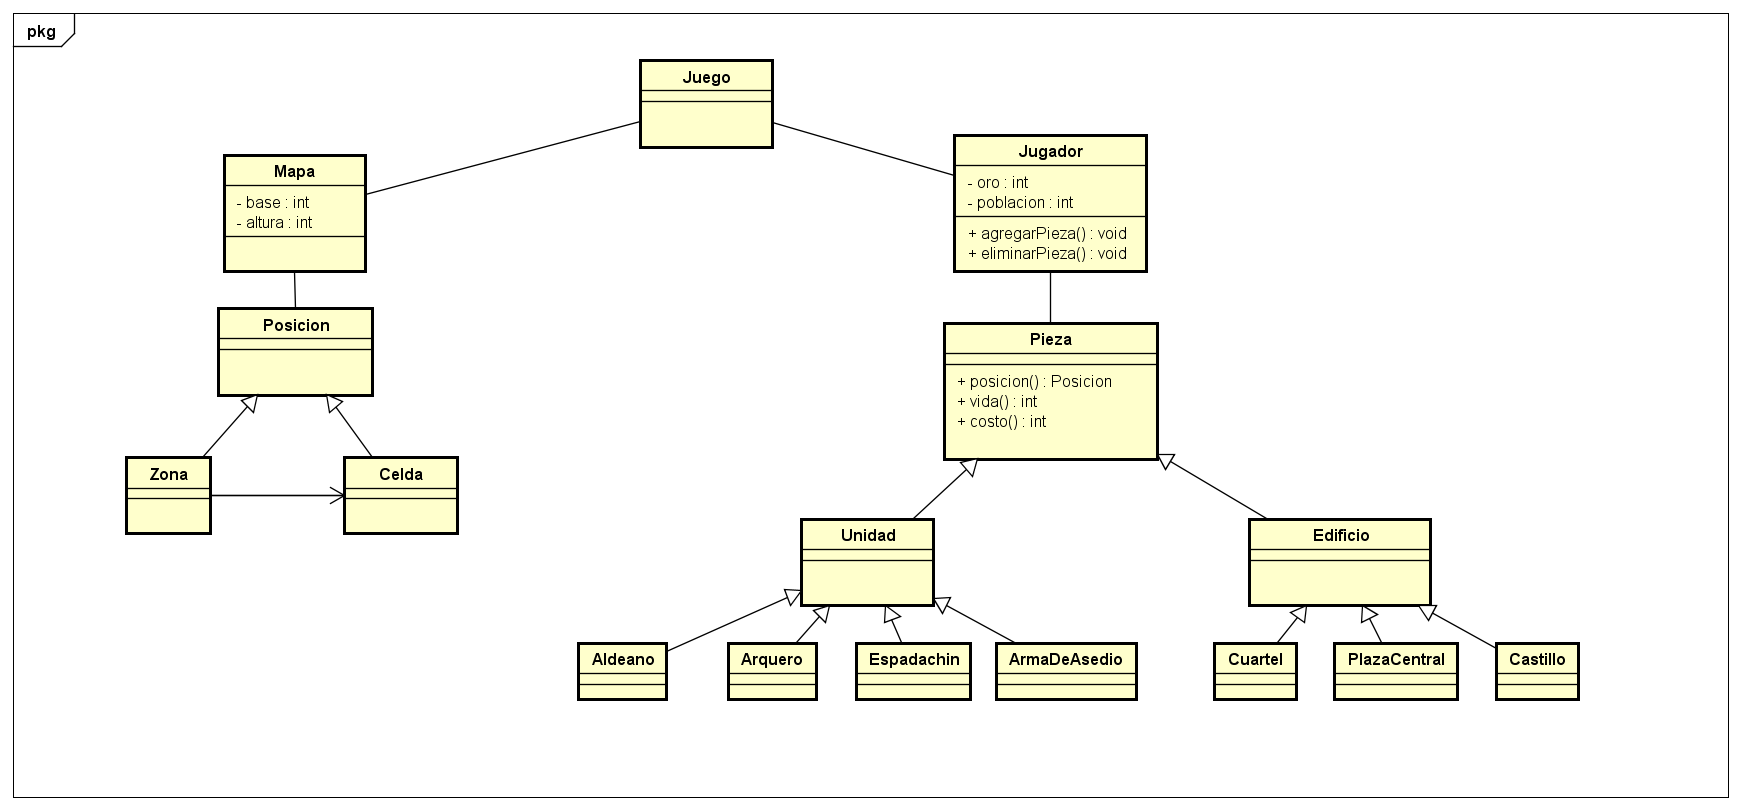
\includegraphics[width=1.15\textwidth]{juego.png}
	\caption{\label{fig:class01}Diagrama de clases }
\end{figure}

Como se observa en el diagrama de clases, el Juego tiene 2 Jugadores, y un mapa. El Mapa contiene Posiciones, que pueden ser Celdas o Zonas (conjunto de Celdas). Por otro lado, cada jugador tiene una cantidad de oro, y una cantidad de unidades (población). Además, cada jugador controla sus Piezas, que pueden ser Unidades (se mueven) o Edificios. Las Unidades en el presente juego pueden ser Aldeano, Arquero, Espadachin o Arma de Asedio. Por otro lado, los Edficios disponibles son Cuartel, Plaza Central o Castillo. Cada Pieza tiene un costo por crearla y una vida que al llegar a cero, desaparece del mapa. 

\begin{figure}[H]
	\centering
	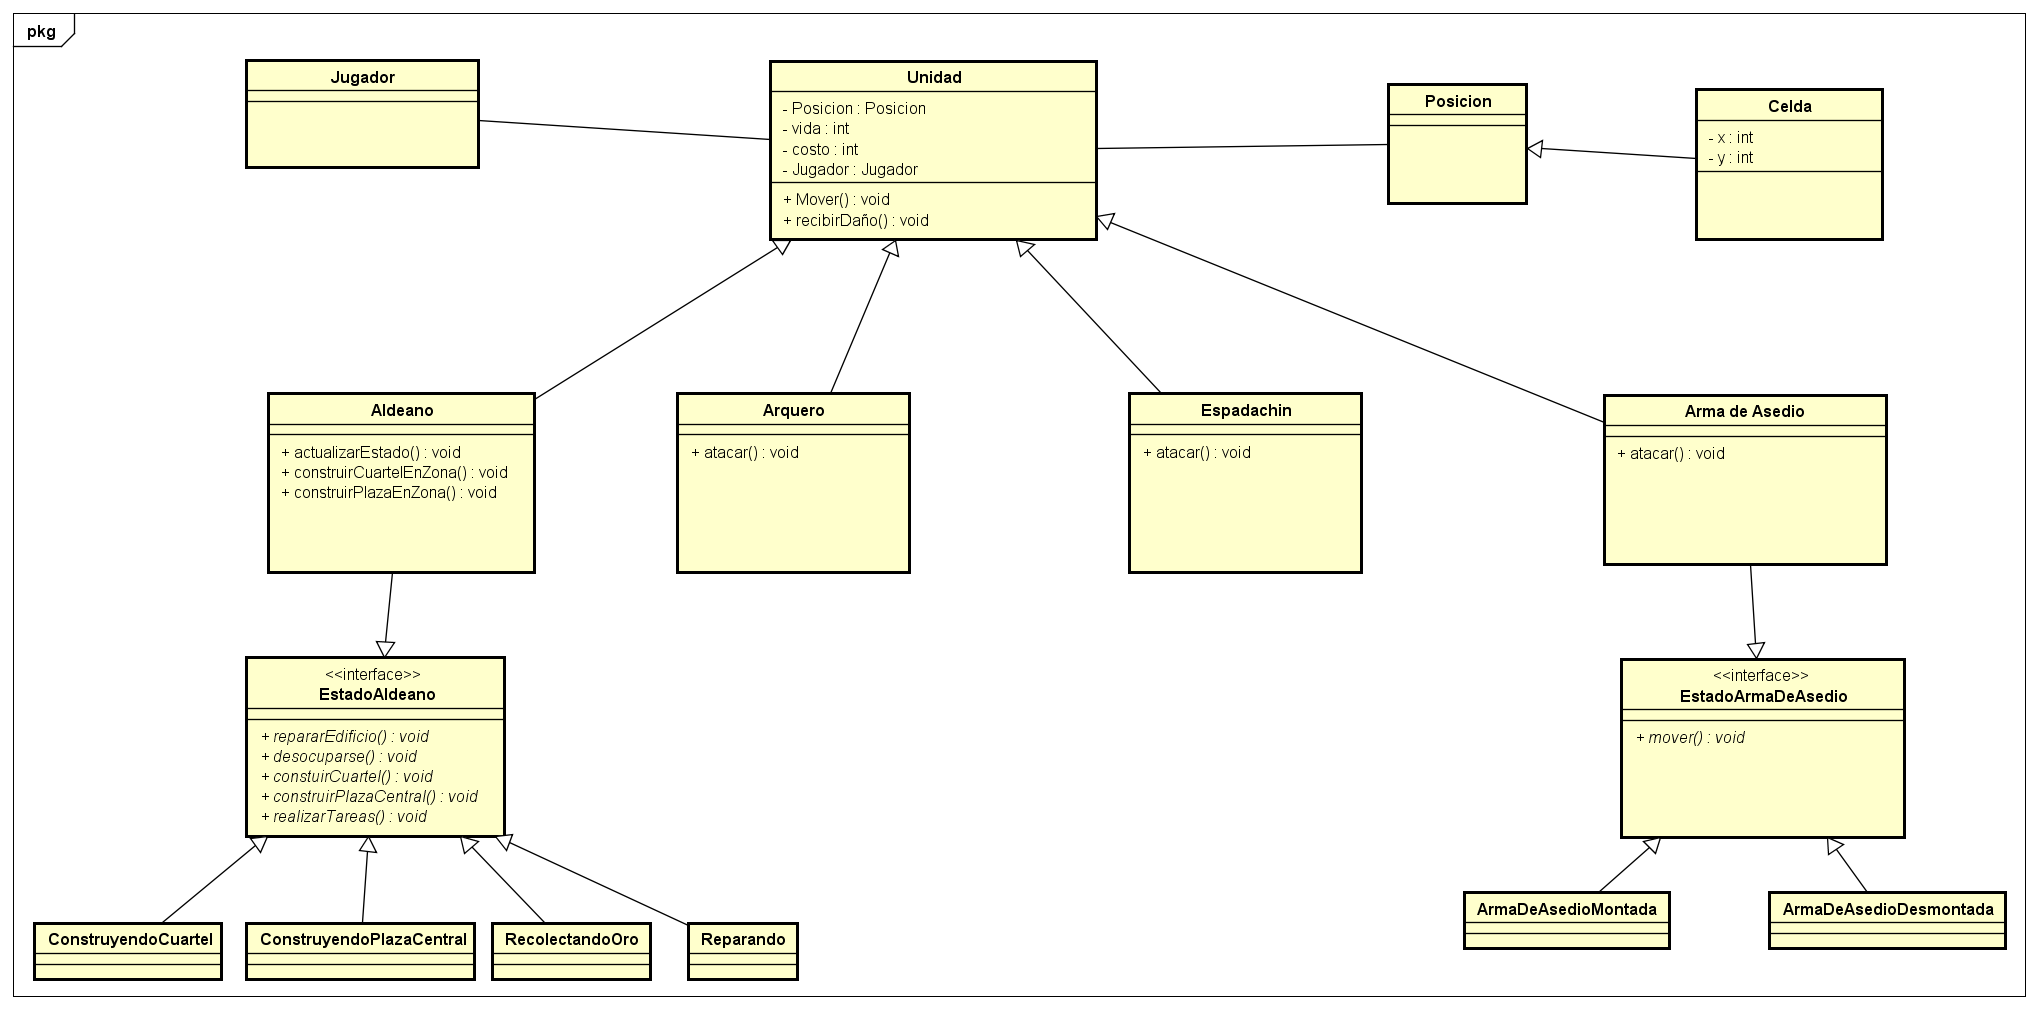
\includegraphics[width=1.15\textwidth]{unidad.png}
	\caption{\label{fig:class01}Diagrama de clases }
\end{figure}

Al centrarnos en la clase Unidad, se observa que cada instancia posee una Posición, que es una celda (x,y). Cada tipo de Unidad puede moverse, pero no todos pueden atacar (el Aldeano no puede). Tanto para la clase Aldeano como Arma de Asedio, como sus acciones dependen de su estado, se utilizó el patrón State. Para el primer caso, hay 4 casos posibles: Aldeano reparando, recolectando oro (libre), construyendo un cuartel o una plaza. Para cada estado, sus acciones son distintas. Para simular un turno, se ejecuta el método realizarTareas. Para el Arma de Asedio, solo puede atacar si esta montada, y solo puede moverse si esta desmontada.  

\begin{figure}[H]
	\centering
	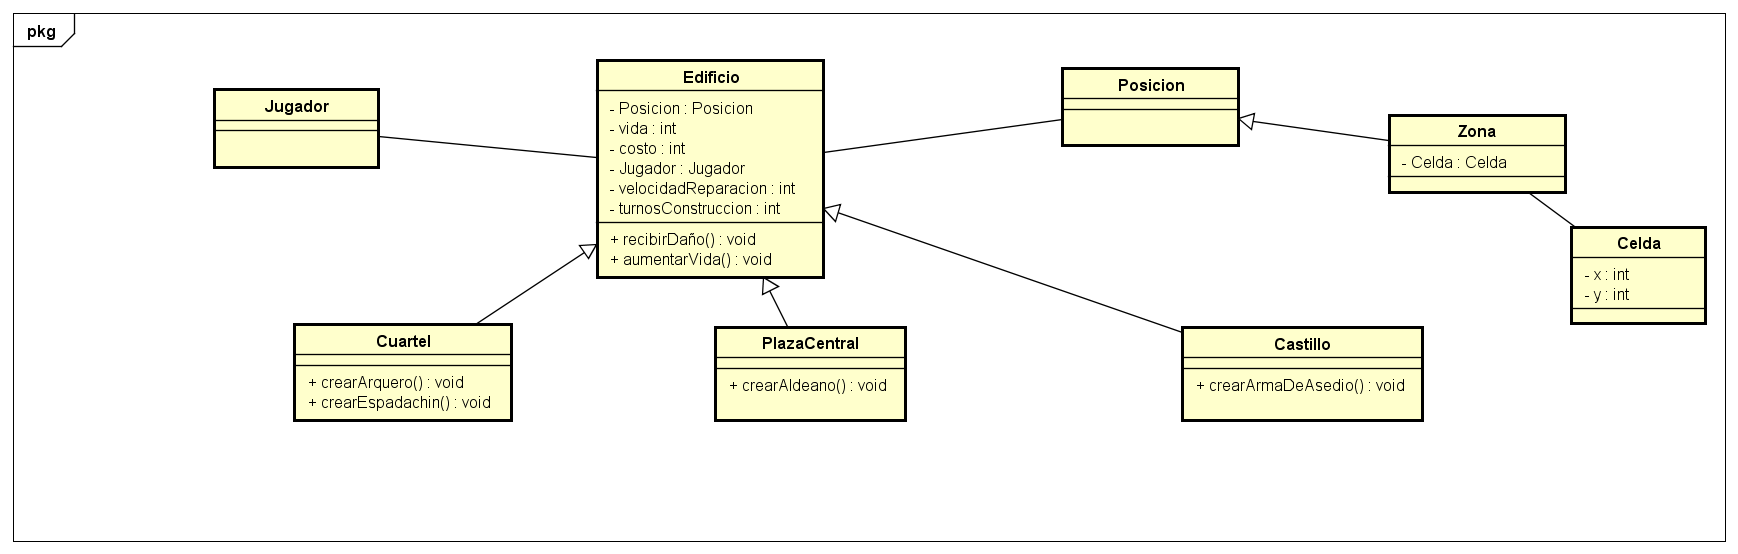
\includegraphics[width=1.15\textwidth]{edificio.png}
	\caption{\label{fig:class01}Diagrama de clases }
\end{figure}

Al analizar la clase Edificio, vemos que su Posicion es una Zona, que es un conjunto de Celdas. Además, los edificios tienen como agregado una velocidad de reparación, y la cantidad de turnos que tardan en construirse. Un Edificio puede ser del tipo Cuartel, PlazaCentral o Castillo. Todos atacan, y todos pueden ser reparados, pero el castillo no puede ser construido.
A su vez, cada edificio crea una Unidad en sus cercanías, pero el tipo de Unidad depende del tipo de Edificio. Por ejemplo, la Plaza Central solo crea Aldeanos. 

\section{Detalles de implementación}\label{sec:implementacion}
% Explicaciones sobre la implementación interna de algunas clases que consideren que puedan llegar a resultar interesantes.

\subsection{Análisis de las principales clases}\bigbreak
\subsubsection{Juego}

Al inicializar la clase Juego, se llama a inicializarJugadores(), lo cual crea dos jugadores, con sus respectivos castillos, plazas y aldeanos, y los coloca en el Mapa en posiciones prefijadas. Luego se simulan los turnos con un loop, hasta que un castillo es destruido totalmente.  

\subsubsection{Jugador}

Al inicializar la clase Jugador, se le asigna la cantidad de oro predefinida (100), y se crean listas de unidades, edificios y aldeanos, donde el jugador lleva la cuenta de sus piezas, y donde las puede manipular. Cada jugador puede agregar o eliminar piezas.

\subsubsection{Mapa}

El mapa tiene un tamaño, dado por una base (int) y una altura (int). Además, posee una lista de posiciones "activas", que indican que ahí se encuentra una pieza. Para esta clase, al ser una sola instancia, se uso el patrón singleton, lo cual permitió no tener que pasarlo por parámetro.

\subsubsection{Posición}

Como cada pieza tiene una posición en el mapa, ésta puede ser una zona o una celda, dependiendo de si es un Edificio o una Unidad. 
Las celdas se implementaron con dos atributos, "X" para la coordenada horizontal e "Y" para la coordenada vertical. 
Tanto las celdas como las zonas tiene muchos métodos que indican si una pieza esta dentro del rango, lo cual es útil a la hora de atacar. 
Para inicializar una Zona, se le indica la celda de origen, que por convención es la celda de arriba a la izquierda, y se le indica las dimensiones. 

\subsubsection{Unidad}
Al crear una unidad, hay que indicar la celda donde se va a colocar, y el jugador a quien le va a pertenecer. 
Las unidades, a diferencia de los edificios, se pueden mover en las 8 posibles direcciones. 
Para el Aldeano, se uso el patron state, permitiendo que cada estado actúe según corresponda. Se presentan 4 estados posibles, todos con el método realizarTareas. Por ejemplo, si el aldeano esta recolectando oro(libre), al ejecutar realizarTareas (1 turno), se le suma 20 de oro al jugador correspondiente. 
Al reparar un edificio, cada turno le manda el mensaje aumentarVida al edificio. Si no es posible aumentar más su vida, se desocupa, es decir, cambia el estado a recolectando oro. 
El límite de unidades es 50, y esto es controlado por la clase jugador.
Para el Arma de Asedio, también se usó el patron state, pero con solo dos estados, montada y desmontada. 

\subsubsection{Edificio}
Para inicializar un Edificio, es necesario indicar la celda origen (arriba a la izquierda) y el jugador correspondiente. 
Un aldeano tarda cierta cantidad de turnos en construirlo, y no puede ser interrumpido durante los mismos. Sin embargo, si un aldeano esta reparando un edificio, sí puede cambiar de tarea, por ejemplo, construir un edificio, si es posible. 
Todos los edificios pueden atacar, pero lo hacen de distinta forma, pues infligen distinto daño. Para esta tarea, se utilizó el patron double dispatch.
Una vez por turno el Castillo ataca a las piezas en rango 3 o menos.


\subsection{Observaciones}



\section{Excepciones}\label{sec:excepciones}
% Explicación de cada una de las excepciones creadas y con qué fin fueron creadas.
Las excepciones ocurren cuando el usuario no cumple con alguna de las pre condiciones establecidas. A continuación se nombras las principales excepciones usadas, pues no se cubrieron todos los casos (como verificar fechas, que semanas sea mayor a 0, etc) pues escapaba del objetivo principal del trabajo.

\begin{description}
\item[RecursoOcupadoError] Esta excepción ocurre cuando un recurso tiene un evento en una fecha, y es agregado a otro evento en esa misma fecha. Sólo puede ocurrir con el mensaje al Calendario: AgregarEvento().

\end{description}

\section{Diagramas de secuencia}\label{sec:diagramasdesecuencia}
% Mostrar las secuencias interesantes que hayan implementado. Pueden agregar texto para explicar si algo no queda claro.

A continuación se muestran algunos diagramas de secuencia de los principales métodos del sistema. En ellos se observa la interacción entre las distintas clases, mostrando el flujo de mensajes enviados.

\begin{figure}[H]
\centering
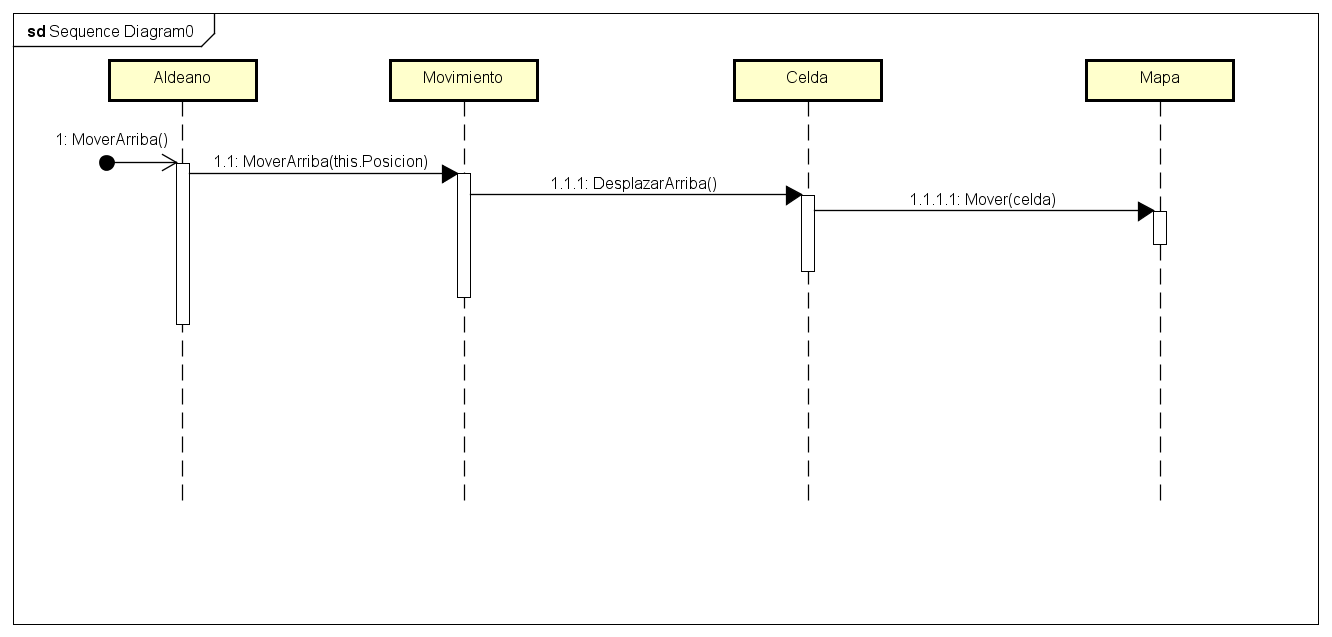
\includegraphics[width=1.15\textwidth]{mover.png}
\caption{\label{fig:seq01}Secuencia de AgregarEvento().}
\end{figure}





\section{Conclusiones}\label{sec:conclusiones}

Escribir


\end{document}
